\chapter{Implementation and Application}
\label{chap:implementation}

\section{Environments and Tools Used}
\label{sec:tools}

The development and training of the student model, in addition to the creation of the mobile application, relied on a set of modern and effective tools and technologies:

\begin{enumerate}
    \item \textbf{PyTorch Framework:} Chosen for its flexibility and ease of use in building and training deep learning models, in addition to its extensive support from the scientific community and available resources.
    \item \textbf{Flutter Development Kit:} Used to build the cross-platform mobile application for both Android and iOS from a single codebase, which simplifies the development and deployment process. It was specifically chosen for its libraries that support running AI models in the ONNX format.
    \item \textbf{VS Code Editor:} An advanced code editor used for writing all the project's source code. Its support for a wide range of languages and features through diverse extensions makes it highly effective.
    \item \textbf{GIT Version Control:} A version control system used to track changes to the software during development. This tool facilitates error detection and rollbacks, allowing us to maintain multiple versions of the program and revert to any of them if needed.
    \item \textbf{ONNX (Open Neural Network Exchange):} An open file format used to run trained artificial intelligence models. Flutter contains libraries that support running models in this format, which was crucial for deploying the model on a mobile device.
    \item \textbf{Teacher Model (Depth Anything V2 Small):} This is the specific, pre-trained "teacher" model used to provide the expertise that is "distilled" to the student model.
    \item \textbf{MobileNetV3 Architecture:} An efficient Convolutional Neural Network (CNN) architecture designed specifically for mobile and resource-constrained devices. It was considered as an encoder for the student model due to its lightweight structure and its ability to achieve a good balance between accuracy and inference speed~\cite{koonce2021mobilenetv3}. This was one of the attempts before adopting the final MobileViT-XS architecture.
    \item \textbf{MobileViT-XS Architecture:} The specific neural network architecture chosen as the encoder for the lightweight student model. It is a hybrid architecture that combines the efficiency of CNNs with the power of Vision Transformers~\cite{mehta2021mobilevit}, making it ideal for mobile devices.
    \item \textbf{Google Colaboratory (Colab):} A cloud-based development environment based on Jupyter notebooks. It was used in this project to train the deep learning model. The platform provided access to high-performance computing resources, specifically Graphics Processing Units (GPUs), which significantly accelerated the model training process and allowed for efficient experimentation with different architectures and configurations without the need for expensive local hardware.
\end{enumerate}

\section{Model Building and Training}
\label{sec:model_building}

\subsection{Environment Setup}
\label{subsec:env_setup}

A dedicated virtual environment was created for the project. This environment contains a specific Python interpreter along with libraries and files isolated from other projects, preventing conflicts between package versions. After activating the environment, all required libraries defined in the \texttt{requirements.txt} file were installed to execute the code for building and training the model.

\subsection{File Structure}
\label{subsec:file_structure}

The project was organized with the following clean file structure:
\begin{description}
    \item[\texttt{Config}:] This folder contains all constants and general information utilized across the project, such as model paths, appropriate image dimensions, transformations applied to images before training and testing, and the selected weighting coefficients for the loss function.
    \item[\texttt{notebooks}:] Contains Jupyter notebooks that were executed on Google Colab for training and testing specific model architectures or loss functions, due to the lack of available local hardware resources.
    \item[\texttt{Models}:] This folder contains the source code for the student and teacher model architectures. Notably, the \textit{Factory} design pattern was used to allow for easily swapping different architectures for the student or teacher. This ensures a clean codebase where only a few lines need to be changed in \texttt{factory.py} and \texttt{config.py}, leaving the files that use the models unchanged.
    \begin{itemize}
        \item \textbf{For the Teacher:} A \texttt{class} was built to wrap the pre-trained model to normalize its output and extract internal feature maps. An image is passed to the pre-trained model, and feature maps from specific layers are extracted to serve as learning targets for the student. These features are then reshaped to a format the student understands (bridging the technical gap between how Transformers and CNNs process information). Finally, the output depth map is normalized so its pixel values are between 0 and 1.
        \item \textbf{For the Student:} Several architectures were tested. The final version is distributed across four classes:
        \begin{itemize}
            \item \texttt{UpsampleBlock}: Defines the upsampling block used in the decoder. It doubles the spatial resolution of the input and uses \textit{Depthwise Separable Convolutions}, which are highly efficient as they significantly reduce the number of computational operations and model size compared to traditional convolutions.
            \item \texttt{FeatureFusionBlock}: Defines the feature fusion block in the decoder. It merges high-level features from the decoder stage with low-level features from the encoder stage, effectively acting as our implementation of skip-connections.
            \item \texttt{MiniDPT}: Represents the decoder. It mimics the decoder used in the teacher model but is much lighter. It projects the feature maps from the encoder to match the decoder's dimensions and is defined recursively with several layers of the two blocks described above. Finally, a prediction head with a \texttt{Sigmoid} activation function is used to output the final depth map with values between 0 and 1.
            \item \texttt{StudentDepthModel}: This class uses the pre-trained encoder (the final design uses MobileViT-XS), extracts internal feature maps from it, passes them to the MiniDPT decoder, and then outputs the final result.
        \end{itemize}
    \end{itemize}
    \item[\texttt{datasets}:] Contains a class for loading the training and testing datasets and applying the desired transformations (\texttt{Transforms}).
    \item[\texttt{data}:] Contains a script to rename images with a numbered naming convention and an \texttt{images} subfolder holding all the images the model was trained on, which were collected with the help of friends.
    \item[\texttt{criterion}:] Here, the loss functions are defined. Due to the need to test several loss functions, the \textit{Factory} and \textit{Strategy} design patterns were used to allow for changing the loss function with great flexibility by modifying a single line in \texttt{config.py}. The primary function used is defined in the \texttt{CombinedDistillationLoss} class, which implements what was theoretically defined in Section~\ref{sec:training_methodology}.
    \item[\texttt{utils}:] Contains helper tools for training and use. It also uses a \textit{Factory} pattern to allow for selecting different optimizers and defines the transformations applied to images before they are fed into the model. It also contains \texttt{metrics.py} for calculating the evaluation metrics for the depth map based on the criteria mentioned in the theoretical study.
    \item[\texttt{scripts}:] This folder contains scripts that perform a complete pipeline:
    \begin{itemize}
        \item A \textbf{training script} that loads the models and dataset, performs the training, and saves the best model based on the loss value on a dedicated validation set.
        \item An \textbf{evaluation script} that shows the model's performance according to the metrics defined in the theoretical study(See Section~\ref{sec:evaluation_metrics}).
        \item An \textbf{inference script} that uses the specified model to generate depth maps for one or more specified images.
        \item A \textbf{conversion script} to convert the model from \texttt{.pth} format to \texttt{.onnx}, which is useful at the deployment stage.
    \end{itemize}
    \item[\texttt{tests}:] This folder contains tests. Unit testing was defined for every module in the program under various edge cases. Afterward, integration testing was performed between these modules by testing a complete, miniature training pipeline.
\end{description}

\subsection{Training Attempts}
\label{subsec:training_attempts}

Several experiments were conducted to improve the model's performance and design. In this phase, training was conducted on a smaller dataset to find the most suitable model before training on a more diverse dataset. The most prominent attempts are summarized below:

\begin{enumerate}
    \item \textbf{Attempt 1: Using MobileNetV3 Encoder}
    The first attempt involved using a \textbf{MobileNetV3-Large} encoder with a simple decoder composed of upsampling and standard convolutional layers. Equal weighting coefficients were used for the components of the loss function.
    \begin{itemize}
        \item \textbf{Observation:} The performance was poor. The resulting depth map, shown in Figure~\ref{fig:attempt1}, lost many details due to the absence of low-level features during the reconstruction process, as shown in Figure~\ref{fig:attempt1}. After this attempt, the loss weights were adjusted to increase the weight of the gradient loss to encourage the model to capture edges, and the SILog loss weight was also increased.
    \end{itemize}

    \begin{figure}[htbp!]
        \centering
        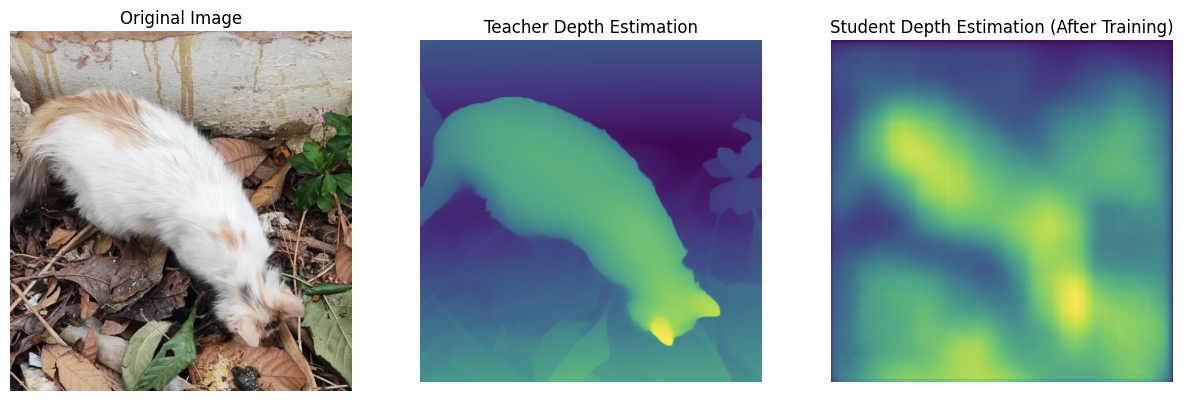
\includegraphics[width=\textwidth]{images/training_attempt_1.png}
        \caption{Results of the First Training Attempt.}
        \label{fig:attempt1}
    \end{figure}
    
    \item \textbf{Attempt 2: Same Encoder with Skip-Connections}
    \begin{itemize}
        \item \textbf{The Architecture:} The same MobileNetV3 architecture was used, but with the addition of skip-connections from different layers in the encoder to the corresponding layers in the decoder.
        \item \textbf{Observation:} A noticeable improvement in the quality of the depth maps was observed (Figure~\ref{fig:attempt2}), as the skip-connections helped in restoring fine spatial details. However, the architecture was still not ideal. The results commonly lacked a sense of \textit{global context}. From this point, we shifted towards using MobileViT as the encoder.
    \end{itemize}

    \begin{figure}[htbp!]
        \centering
        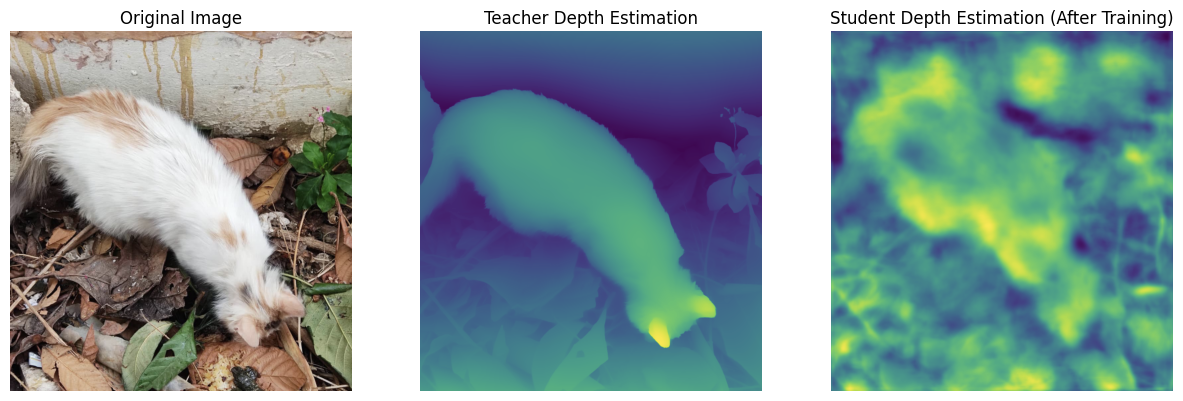
\includegraphics[width=\textwidth]{images/training_attempt_2.png}
        \caption{Results of the Second Training Attempt.}
        \label{fig:attempt2}
    \end{figure}

    \item \textbf{Attempt 3 (Final Model): Using MobileViT}
    This attempt represents the final and best-performing architecture that was adopted.
    \begin{itemize}
        \item \textbf{The Architecture:} The encoder was replaced with \textbf{MobileViT-XS}, and the decoder was the custom \textbf{MiniDPT} described in the file structure section.
        \item \textbf{Training Details:}
        \begin{itemize}
            \item \textbf{Dataset:} Unlabeled images taken with a mobile phone camera.
            \item \textbf{Data Augmentation:} To increase data diversity and prevent overfitting, operations such as horizontal flipping, random rotation, cropping, resizing, and color jittering were applied.
            \item \textbf{Optimizer:} The \textbf{AdamW} optimizer was used with a \textbf{CosineAnnealingLR} learning rate scheduler to dynamically adjust the learning rate during training, which helps in reaching a better convergence point.
            \item \textbf{Loss Function:} The composite loss function was used with the weights shown in Table~\ref{tab:loss_weights}.
        \end{itemize}
    \end{itemize}

    \begin{table}[htbp!]
        \centering
        \caption{Weighting Coefficients for the Composite Loss Function.}
        \label{tab:loss_weights}
        \begin{tabular}{lcccc}
            \toprule
            \textbf{Weight} & $\lambda_{\text{silog}}$ & $\lambda_{\text{grad}}$ & $\lambda_{\text{feat}}$ & $\lambda_{\text{attn}}$ \\
            \midrule
            \textbf{Value}  & 1.5 & 1.5 & 0.5 & 0.4 \\
            \bottomrule
        \end{tabular}
    \end{table}

    \begin{itemize}
        \item[]
        \begin{itemize}
            \item \textbf{Epochs:} The model was trained for \textbf{60 epochs}. An initial learning rate of \textbf{$10^{-3}$} was used for the decoder and \textbf{$10^{-5}$} for the pre-trained encoder.
            \item \textbf{Batch Size:} A batch size of \textbf{12} was used with an image resolution of \textbf{384 x 384} pixels.
            \item \textbf{Observation:} We witnessed a significant improvement in the results, with a better understanding of the global context and an ability to capture edges. However, the model is susceptible to color-based artifacts, occasionally misinterpreting color variations as changes in depth, as seen with the liquid on the wall in Figure~\ref{fig:attempt3}. This limitation likely stems from a lack of diversity or inherent biases in the training data.
        \end{itemize}
    \end{itemize}

    \begin{figure}[htbp!]
        \centering
        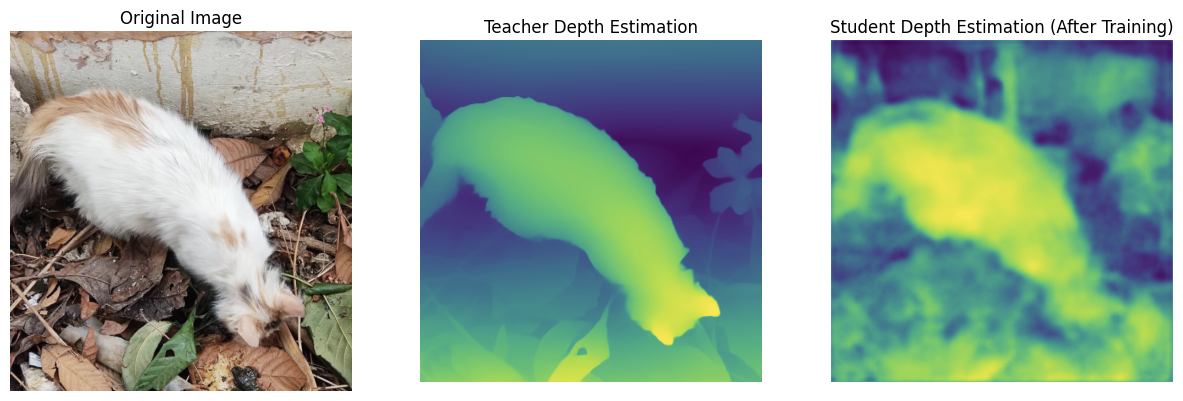
\includegraphics[width=\textwidth]{images/training_attempt_3.png}
        \caption{Results of the Third Training Attempt.}
        \label{fig:attempt3}
    \end{figure}
    
    This model was adopted, and the final training process was conducted on a larger dataset.
\end{enumerate}

\subsection{Tuning the Loss Function Weights}
\label{subsec:loss_tuning}

Initially, equal weights were used for the loss components, but this led to blurry results around the edges, as shown in Figure~\ref{fig:loss_tuning}.

\begin{figure}[htbp!]
    \centering
    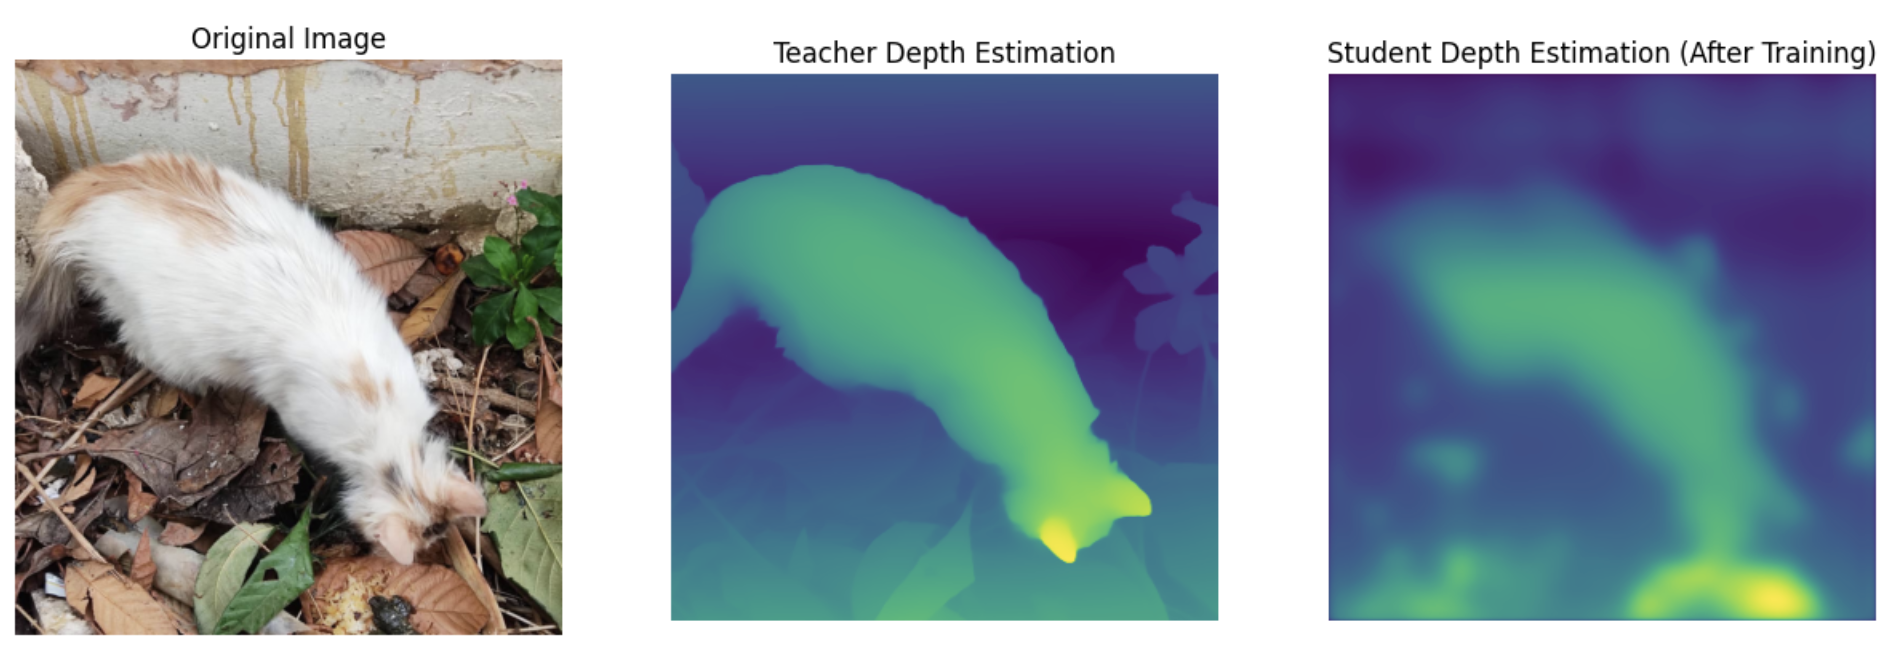
\includegraphics[width=\textwidth]{images/loss_tuning_result.png}
    \caption{Comparison of outputs when using equal weights for loss functions.}
    \label{fig:loss_tuning}
\end{figure}

Based on this, the weight of the gradient loss was gradually increased from 1.0 to 1.5, which showed a marked improvement in preserving details in the validation images. From the same figure, it was also observed that the student model did not focus on the leaves on the left side of the image. This might be because the student was focusing on the main element in the image, which causes the largest activation in the teacher's feature maps, while neglecting other regions. Therefore, the weight of the attention loss was gradually decreased to allow the student to focus on other areas that the teacher might consider secondary. The weight for the primary loss (the scale-invariant logarithmic loss) was increased because it is the core component, and we want the model to learn this primary task well.

\subsection{The Final Training Process}
\label{subsec:final_training}

The model was trained on \textbf{3500} images from the \textbf{COCO} dataset, which is designated for object recognition. However, in our case, we do not need labeled data, as the teacher model effectively "labels" the images by producing a depth map that the student learns from. This dataset also provides a diverse set of images, including both \textbf{indoor} and \textbf{outdoor} scenes.

\begin{figure}[htbp!]
    \centering
    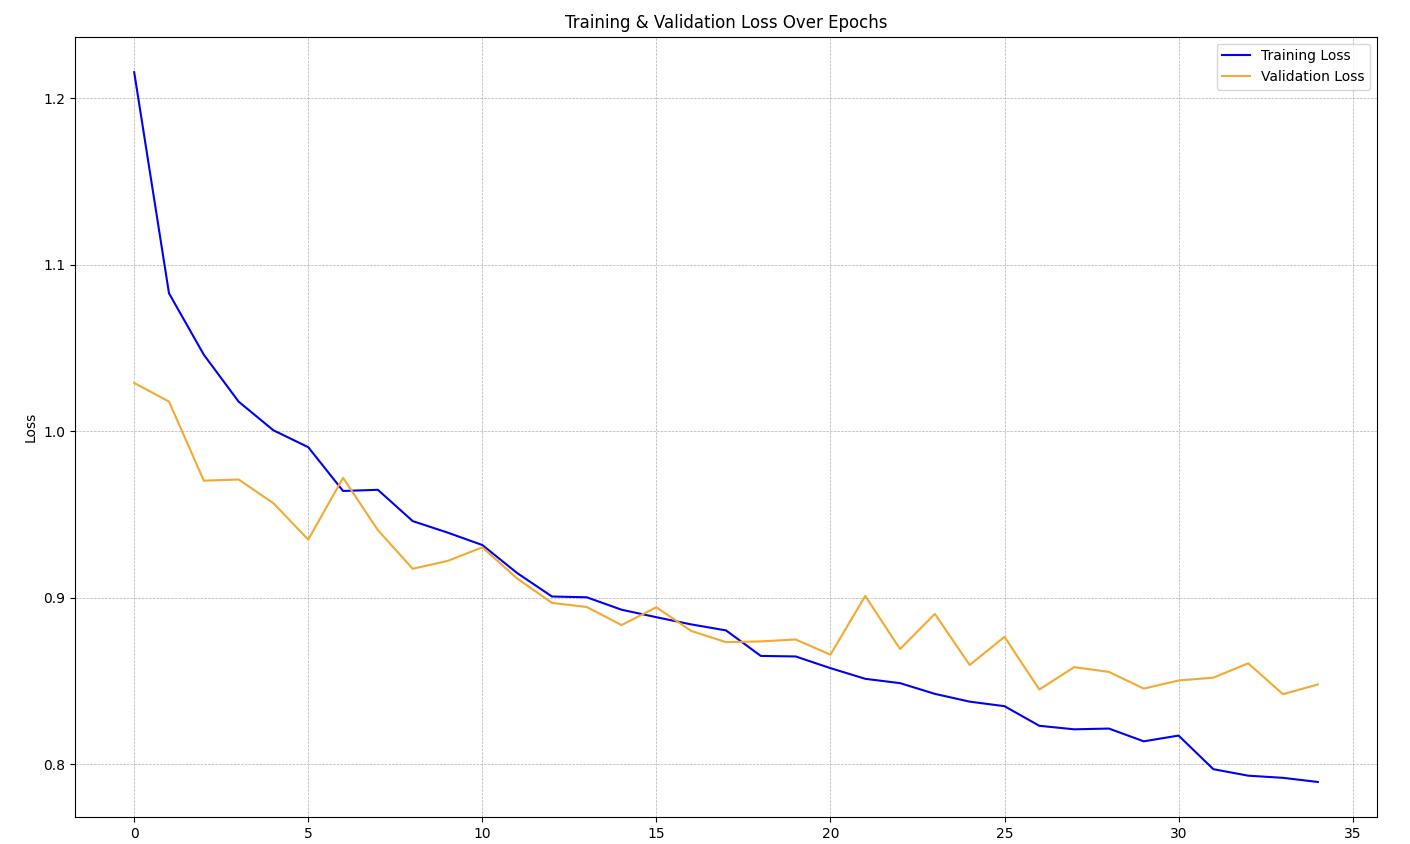
\includegraphics[width=0.8\textwidth]{images/training_loss_graph.png}
    \caption{The loss function for the final training process.}
    \label{fig:loss_graph}
\end{figure}

Training was stopped after epoch 34 to avoid overfitting on the training. The Figure~\ref{fig:loss_graph} shows the loss function on the traning and validation sets as the model trains. This model is evaluated in the quantitative and qualitative evaluation sections in Chapter~\ref{chap:results}.

\section{Mobile Application}
\label{sec:mobile_app}

To demonstrate the practical viability of the developed student model and to confirm that it meets the performance requirements on resource-constrained devices, a Proof of Concept mobile application was developed. As mentioned previously, the application was developed using the \textbf{Flutter} framework.

\subsection{Architecture}
\label{subsec:app_arch}

The application followed an architecture based on the separation of responsibilities to ensure ease of maintenance and future development. The key components are:
\begin{description}
    \item[State Management:] The \texttt{Provider} package with the \texttt{ChangeNotifier} pattern was used to manage the application's state centrally and effectively. This approach separates the business logic from the UI, where the UI listens for changes in the application state and automatically updates itself upon any change (such as selecting a new image or the completion of the processing).
    \item[Services:] The core logic was encapsulated in an isolated service layer.
    \begin{itemize}
        \item \textbf{Model Loader Service:} Responsible for loading the ONNX model from the application's assets. This service activates available Hardware Acceleration (such as NNAPI on Android and CoreML on iOS) to ensure maximum possible performance.
        \item \textbf{Depth Estimator Service:} Contains the complete logic for the depth estimation process, from image preprocessing to applying colormaps to the model's final output.
    \end{itemize}
    \item[Utils:] Helper tools required by the services.
    \item[UI (User Interface):] The UI was built from a collection of independent and reusable \texttt{Widgets}, which are then used in the display screens, making the codebase more organized and clear.
\end{description}

\subsection{Performance Optimizations}
\label{subsec:app_optimizations}

To achieve the primary performance requirement of real-time responsiveness and to avoid freezing the UI during computationally intensive operations, two main optimizations were implemented:
\begin{itemize}
    \item \textbf{Using onnxruntime:} This specialized library was relied upon for running AI models on mobile devices, as it provides the best possible performance by leveraging local hardware capabilities.
    \item \textbf{Background Processing (Isolates):} Both the image preprocessing (resizing, normalization) and the depth map post-processing (applying a colormap) are computationally intensive. To avoid blocking the main thread responsible for UI smoothness, these two operations were moved to be executed in separate background threads (\texttt{Isolates}) using the \texttt{compute} function provided by Flutter. This approach ensures the application remains fully responsive even while processing images.
\end{itemize}

\subsection{Application Features Showcase}
\label{subsec:app_features}

The application provides a simple and intuitive interface that allows the user to perform the following functions:
\begin{itemize}
    \item \textbf{Select an Image:} The user can capture a new photo using the camera or select an existing one from the gallery (See Figure~\ref{fig:app_screenshots1}).
    \item \textbf{Estimate Depth:} A dedicated button starts the depth estimation process, displaying a "Processing..." indicator to provide the user with visual feedback.
    \item \textbf{Display Results:} The original image and the resulting depth map are displayed on the same screen for immediate comparison (See Figure~\ref{fig:app_screenshots1}).
    \item \textbf{Measure Performance:} The inference time taken by the model is displayed in milliseconds below the depth map, providing a direct quantitative measure of the model's efficiency (See Figure~\ref{fig:app_screenshots1}).
    \item \textbf{Customize Display:} The user can change the colormap applied to the output (e.g., from grayscale to Viridis) to get a better visualization of the depth differences (See Figure~\ref{fig:app_screenshots2}).
    \item \textbf{Live Depth Camera:} A live camera feature provides real-time depth estimation at approximately \textbf{4 frames per second} (See Figure~\ref{fig:app_screenshots2}).
    \item \textbf{Night Mode:} The application also includes support for a dark/night mode (See Figure~\ref{fig:app_screenshots2}).
\end{itemize}

\begin{figure}[htbp!]
    \centering
    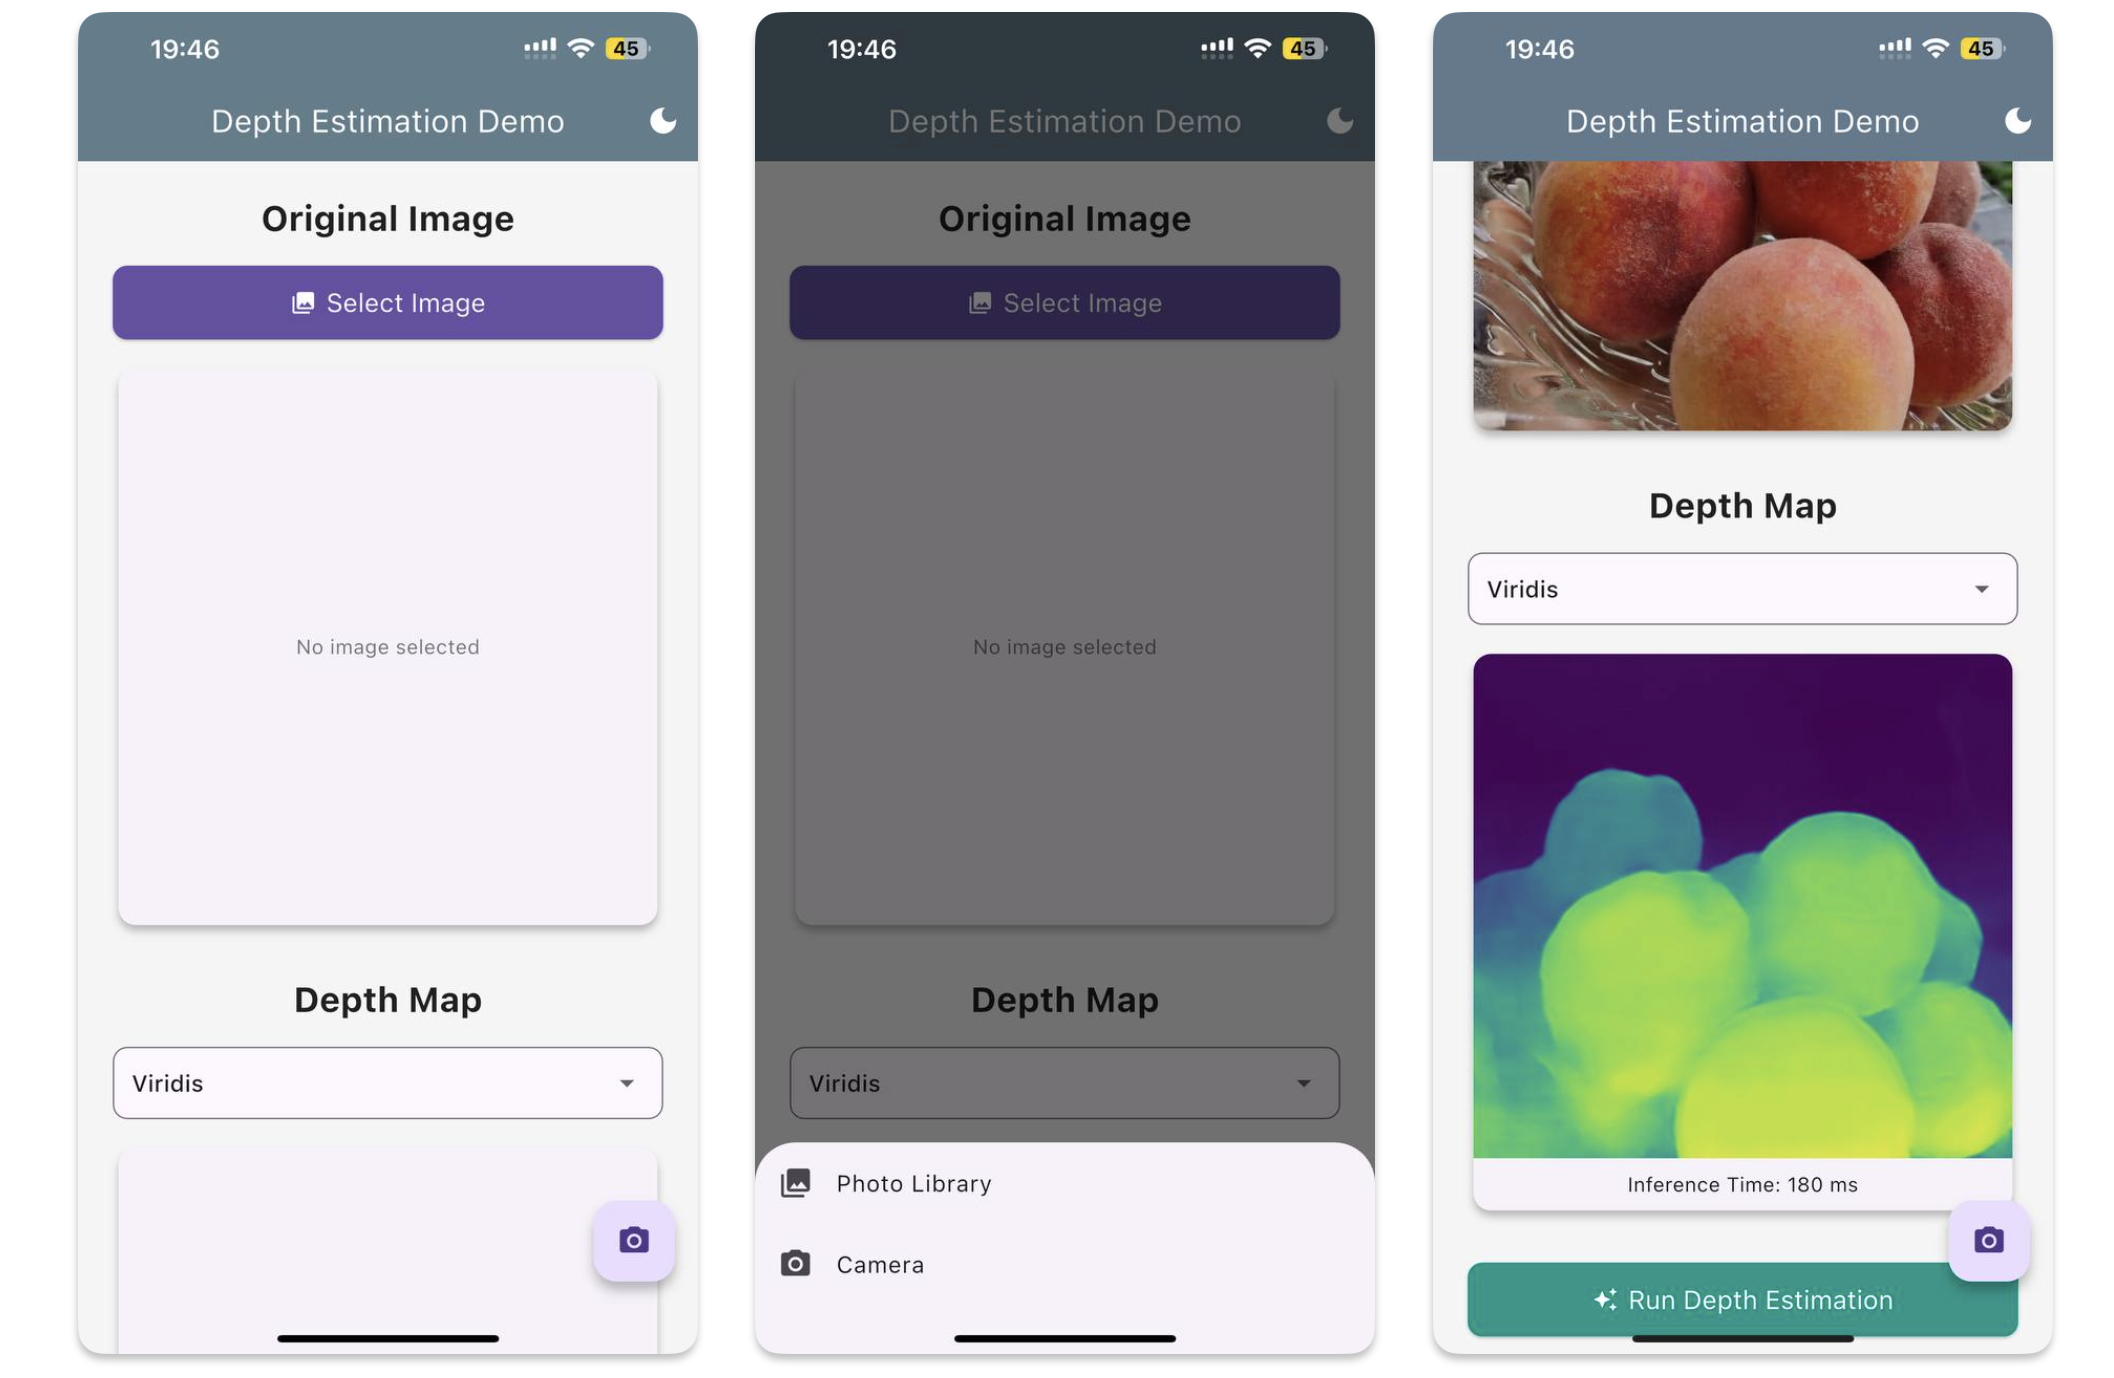
\includegraphics[width=0.9\textwidth]{images/app_screenshots_1.png}
    \caption{Image selection and result display.}
    \label{fig:app_screenshots1}
\end{figure}

\begin{figure}[htbp!]
    \centering
    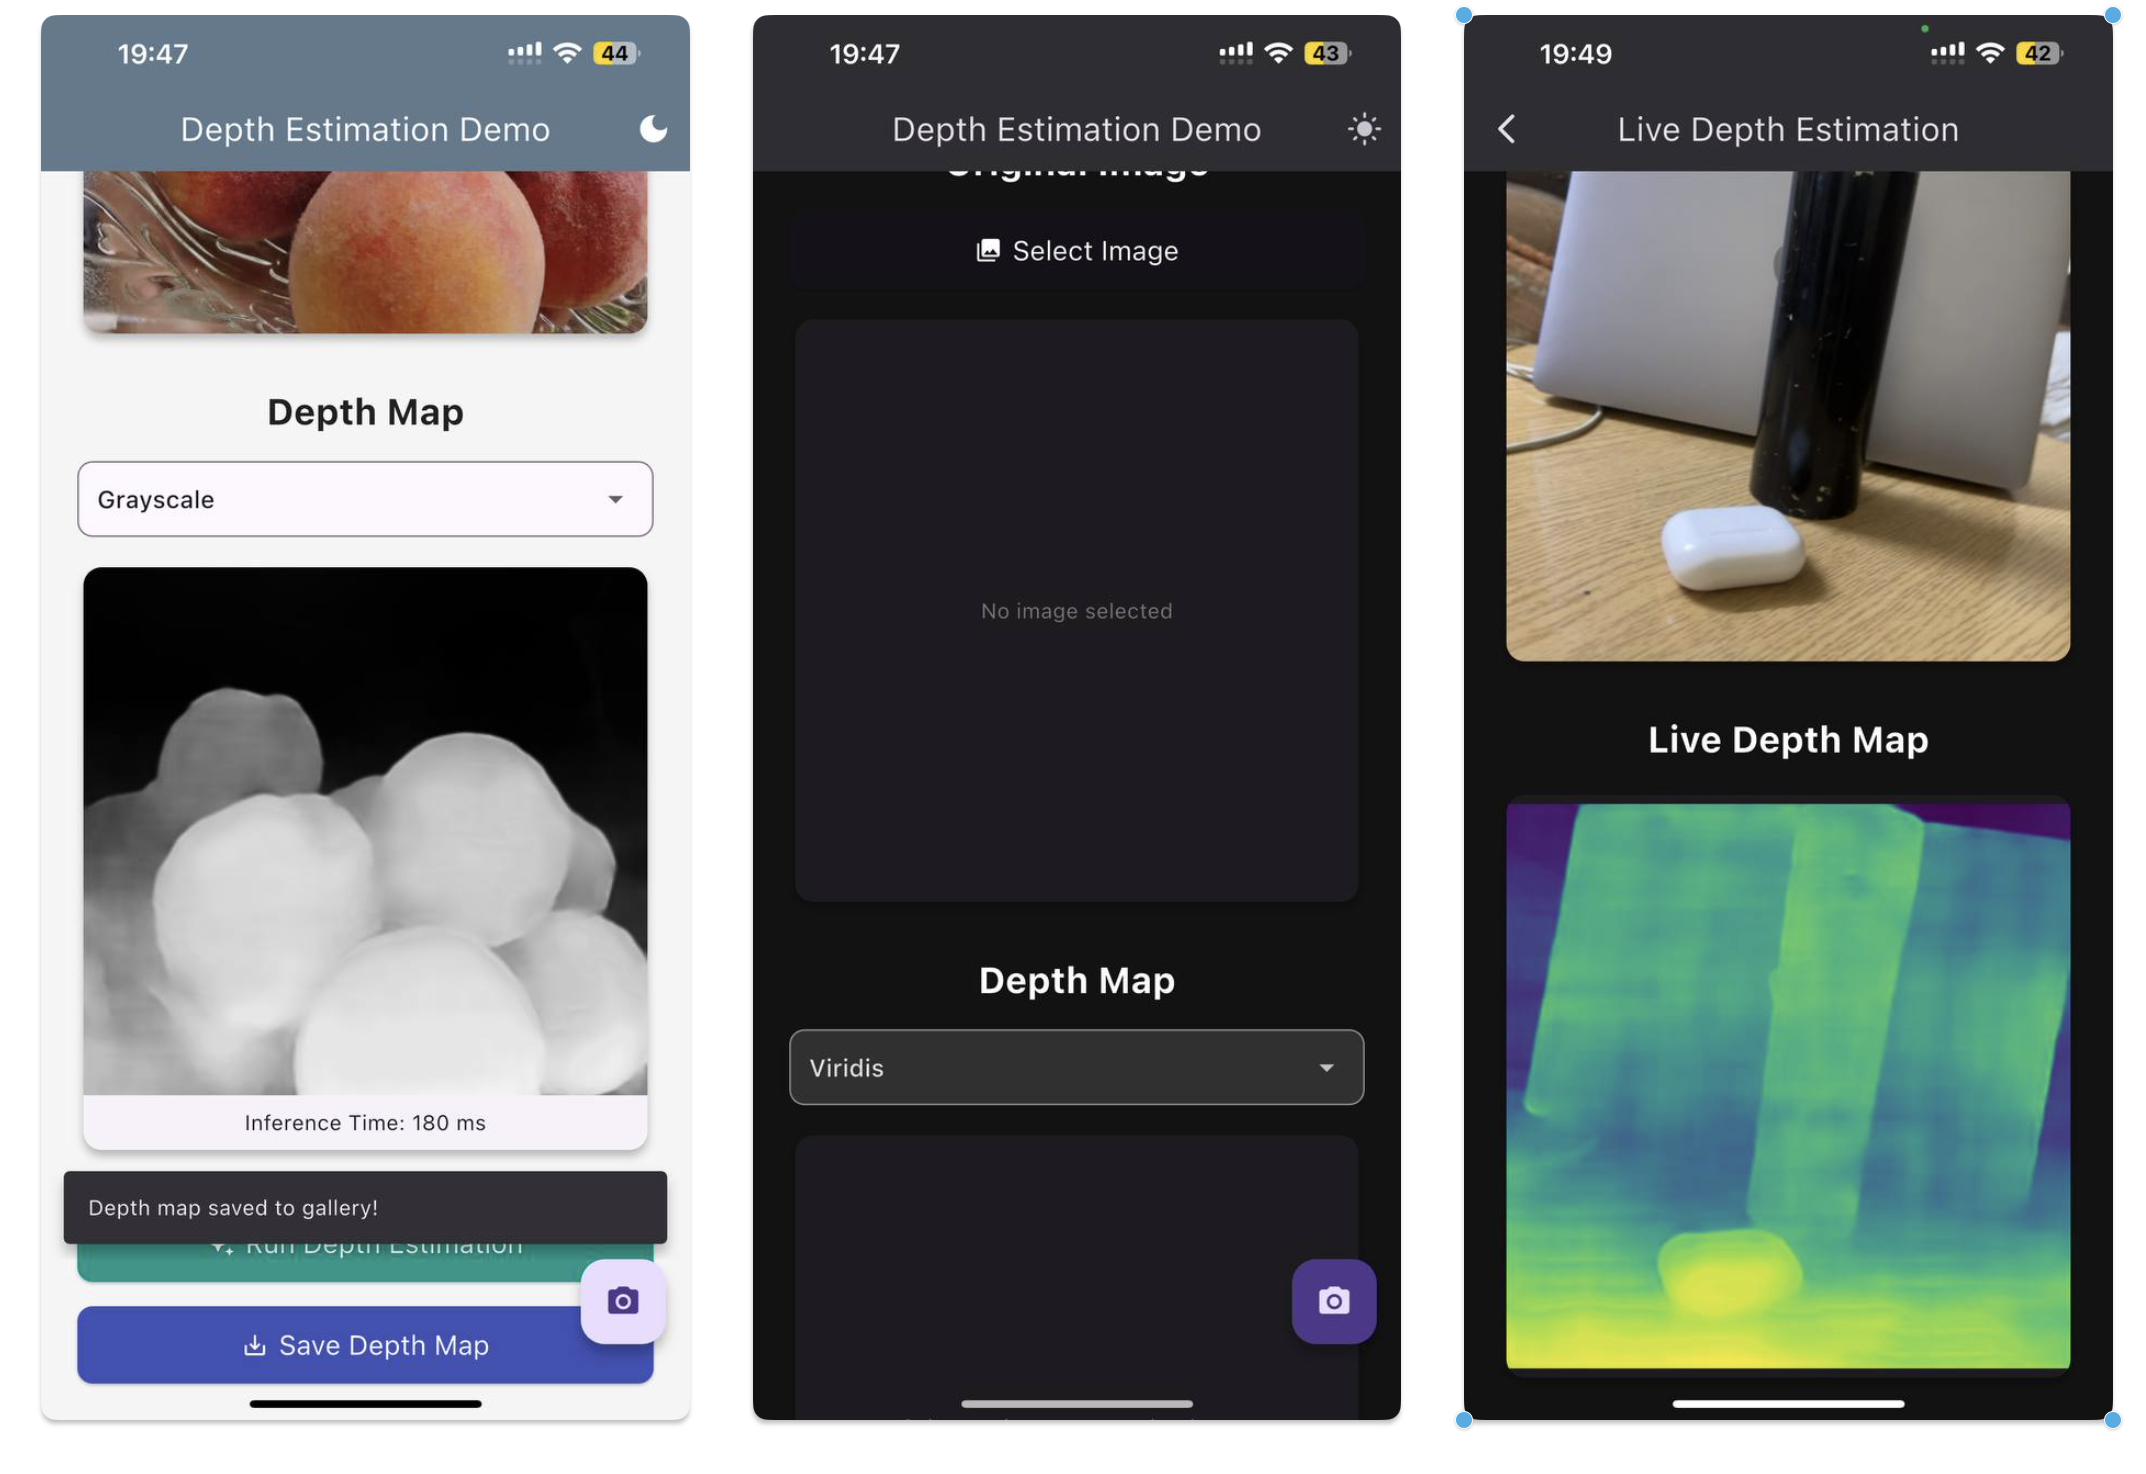
\includegraphics[width=0.9\textwidth]{images/app_screenshots_2.png}
    \caption{Live depth camera, saving the depth map, and depth visualization.}
    \label{fig:app_screenshots2}
\end{figure}

As Shown in Figure~\ref{fig:app_screenshots1} the inference time does not exceed 200 ms, which was one of our goals. Thus, the application successfully proves the effectiveness of the distilled model and its capability to run efficiently in a real-world runtime environment on mobile phones, achieving the specified goals and requirements.